In this section, we provide a brief overview of Graphics processing unit (GPU) by explaining its architecture and working. It is then followed by the background of the applied programming models in the GPU. This background provides required technical knowledge for understanding GPU internal workings which would be helpful while explaining GPU-accelerated database systems.

\subsection*{Graphics Processing Unit (GPU)}
A Graphics processing Unit (GPU) is a specialized electronic device which is initially designed with the purpose of generating output frames intended to display on some output device. It can now be used as the general computation device for performing several heavy computational operations in diverse multi-threaded environments, which is primarily called GPGPU\footnote{General purpose graphics processing unit}. These GPUs have immense processing power due to their huge bandwidth and extreme speed for solving floating point operations as compared to CPUs, which is shown in Figure \ref{fig:gpu_comp}.

\begin{figure}[ht]
\centering
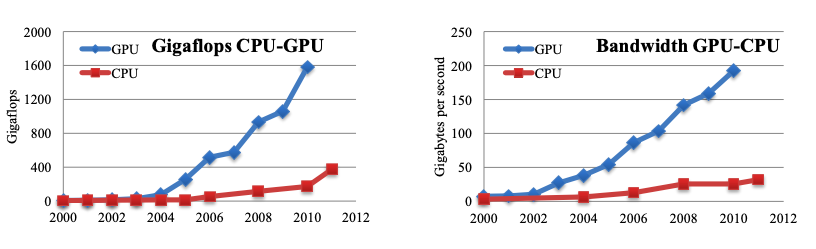
\includegraphics[width=\textwidth]{common/cpu_vs_gpu_speed_comp}
\caption{Comparison of performance for NVIDIA GPUs and Intel CPUs, taken from \cite{gpu_comparison}}
\label{fig:gpu_comp}
\end{figure}

\subsection*{GPU Architecture}
Figure \ref{fig:gpu_arch} shows the architecture of a general modern computer system installed with a graphics card. The graphics card, which is an external device, is connected to the host system using PCI express\footnote{Peripheral Component Interconnect express(PCIe) - interface for connecting high-speed components} bus. This bus can provide data transfer speed of around 16 gbps from host system main memory to graphics card device memory. Due to this limited speed, PCIe bus becomes a major bottleneck for GPU-acceleration which we will see in later sections.

The graphics card contains its own device memory and typically it cannot access host system's main memory. GPU can only interact with graphics card device memory due to which data is required to be transferred from host's main memory to device memory using low-bandwidth bus. Some vendors such as NVIDIA provides a concept of pinned memory, which enables GPU to directly access main memory of the host.

The GPU itself contains several small multiprocessors which uses on-chip shared memory with memory controllers and instructor decoders. Due to these several multiprocessors, GPU provide extreme multi-threaded processing environment which enables tasks to perform heavy computations in small interval of time.
\begin{figure}[ht]
\centering
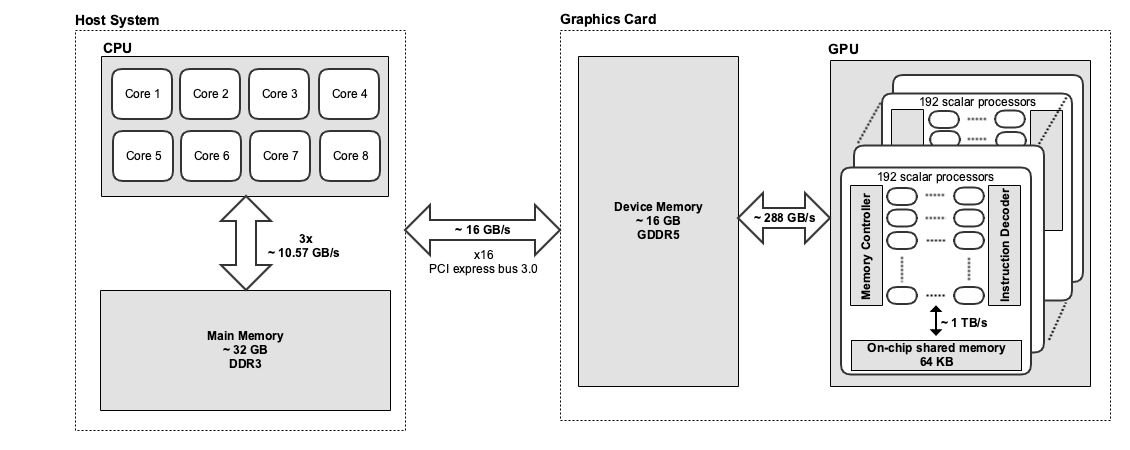
\includegraphics[width=\textwidth]{common/gpu_architecture}
\caption{Exemplary architecture of a system with a graphics card, adapted from \cite{gpu_architecture}}
\label{fig:gpu_arch}
\end{figure}

\subsection*{GPU Programming}
Programs that run on the graphics card works on kernel programming model. Programs in this model consists of host code and kernel\cite{gpu_architecture}, where host code manages the program execution and kernel forms the basic unit of parallelism for harnessing GPU's multi-threaded power. Host code is also responsible for managing data transfer requirements, scheduling program's execution on the device and maintaining state of the code. While invocation, each kernel which is then called a \emph{thread}, executes the host code on its own share of the input and all threads running on the same multiprocessors are logically grouped into a \emph{workgroup}.

Since the beginning of concept of performing general purpose computing on the GPUs, there had been several programming languages that helps us to write kernel programming models for executing jobs on the GPU. It was used to cumbersome and error prone at the early stages, but with the coming of vendor specific general languages to handle such heavy operations, GPGPU jobs implementation has grown immensely. Today, the predominant general purpose languages for GPU kernel programming are NVIDIA CUDA, DirectCompute and OpenCL.
